\documentclass[11pt, oneside]{article}   	% use "amsart" instead of "article" for AMSLaTeX format
\usepackage[margin=1in]{geometry}                		% See geometry.pdf to learn the layout options. There are lots.
\geometry{letterpaper}                   		% ... or a4paper or a5paper or ... 
%\geometry{landscape}                		% Activate for rotated page geometry
%\usepackage[parfill]{parskip}    		% Activate to begin paragraphs with an empty line rather than an indent
\usepackage{graphicx}				% Use pdf, png, jpg, or eps§ with pdflatex; use eps in DVI mode
								% TeX will automatically convert eps --> pdf in pdflatex		
\usepackage{amssymb}
\usepackage{courier}
%usepackage{undertilde}
\usepackage[numbered,framed]{matlab-prettifier}
\usepackage{framed}

\usepackage[T1]{fontenc}
\usepackage{mathtools}  % loads »amsmath«
\usepackage{physics}
\usepackage{listings}

\lstset{
  language=C,                % choose the language of the code
  numbers=left,                   % where to put the line-numbers
  stepnumber=1,                   % the step between two line-numbers.        
  numbersep=5pt,                  % how far the line-numbers are from the code
  backgroundcolor=\color{white},  % choose the background color. You must add \usepackage{color}
  showspaces=false,               % show spaces adding particular underscores
  showstringspaces=false,         % underline spaces within strings
  showtabs=false,                 % show tabs within strings adding particular underscores
  tabsize=2,                      % sets default tabsize to 2 spaces
  captionpos=b,                   % sets the caption-position to bottom
  breaklines=true,                % sets automatic line breaking
  breakatwhitespace=true,         % sets if automatic breaks should only happen at whitespace
  title=\lstname,                 % show the filename of files included with \lstinputlisting;
}

\setlength{\parskip}{0.5em}

%SetFonts
\newcommand\Rey{\mbox{\textit{Re}}}

\title{\vspace{-6ex}\large PHYS 516: Methods of Computational Physics \\
  \normalsize ASSIGNMENT 5- Quantum Dynamics Basics\vspace{-3ex}}
\author{Anup V Kanale}
\date{\vspace{-3ex}\today}							% Activate to display a given date or no date

\begin{document}
\vspace{-6ex}\maketitle
\section{Exponentiation of the Kinetic Energy operator}
From the lecture notes, the Kinetic energy operator is given as
\begin{align}
T &= \left[
\begin{array}{ccccccccc}
2a & b & & & & & b\\
b & 2a & b \\
  & b & 2a & b \\
  &  & \ddots & \ddots & \ddots \\
 & &  & b & 2a & b \\
 & &  &  & b & 2a & b \\
b & &  &  &   & b & 2a
\end{array}\right] \\
&= \frac{1}{2} \left[
\begin{array}{ccccccccc}
a & b & & & & & \\
b & a &  \\
  &  & a & b \\
    &  & b & a \\
  &  & \ddots & \ddots & \ddots \\
 & &  &  &  &  \\
 & &  &  &  & a & b \\
 & &  &  &   & b & a
\end{array}\right] +
\left[
\begin{array}{ccccccccc}
a & & & & & & & b \\
& a & b & & & & & \\
& b & a &  \\
  & & & a & b \\
   & &  & b & a \\
 & & & & \ddots & \ddots & \ddots \\
& & &  &  &  & a & b \\
& & &  &  &   & b & a \\
b & & &  &  &   &  & & a
\end{array}\right] +
\frac{1}{2} \left[
\begin{array}{ccccccccc}
a & b & & & & & \\
b & a &  \\
  &  & a & b \\
    &  & b & a \\
  &  & \ddots & \ddots & \ddots \\
 & &  &  &  &  \\
 & &  &  &  & a & b \\
 & &  &  &   & b & a
\end{array}\right]
\end{align}

We can exponentiate this kinetic energy operator using the Trotter expansion as follows
\begin{equation}
 e^{-iT \Delta t} = U_X^{half} U_x^{full} U_X^{half} + O(\Delta t^3)
\end{equation}

Since T is a sum of block diagonal matrices, each block may be exponentiated individually.
Consider the diagonal block $A = \begin{bmatrix}
a && b \\
b && a
\end{bmatrix}$. From HW1, we know that  A can be diagonalized and expressed as
\begin{equation}
A = \begin{bmatrix}
a && b \\
b && a
\end{bmatrix} = 0.5 \begin{bmatrix}
1 && 1 \\
1 && -1
\end{bmatrix} \begin{bmatrix}
a+b && 0 \\
0 && a-b
\end{bmatrix} \begin{bmatrix}
1 && 1 \\
1 && -1
\end{bmatrix}
\end{equation}
Using telescoping,
\begin{align}
A^n &= 0.5 \begin{bmatrix}
1 && 1 \\
1 && -1
\end{bmatrix} \begin{bmatrix}
(a+b)^n && 0 \\
0 && (a-b)^n
\end{bmatrix} \begin{bmatrix}
1 && 1 \\
1 && -1
\end{bmatrix} \\
&= 0.5\begin{bmatrix}
(a+b)^n + (a-b)^n && (a+b)^n - (a-b)^n \\
(a+b)^n - (a-b)^n && (a+b)^n + (a-b)^n
\end{bmatrix}

\lstinputlisting[language=C, frame=single]{qd1Spectral.c}

\end{align}
Using the definition of exponential, we can write
\begin{align}
e^{i A \Delta t} &= \sum\limits_n \frac{i \Delta t}{n!} A^n \\
	&= \sum\limits_n \frac{i \Delta t}{n!} \frac{1}{2} \begin{bmatrix}
(a+b)^n + (a-b)^n && (a+b)^n - (a-b)^n \\
(a+b)^n - (a-b)^n && (a+b)^n + (a-b)^n
\end{bmatrix} \\
	&= \frac{1}{2} \begin{bmatrix}
\sum\limits_n \frac{i \Delta t}{n!} (a+b)^n + \sum\limits_n \frac{i \Delta t}{n!} (a-b)^n && \sum\limits_n \frac{i \Delta t}{n!} (a+b)^n - \sum\limits_n \frac{i \Delta t}{n!} (a-b)^n \\
\sum\limits_n \frac{i \Delta t}{n!} (a+b)^n - \sum\limits_n \frac{i \Delta t}{n!} (a-b)^n && \sum\limits_n \frac{i \Delta t}{n!} (a+b)^n + \sum\limits_n \frac{i \Delta t}{n!} (a-b)^n
\end{bmatrix} \\
	&= \frac{1}{2} \begin{bmatrix}
	e^{i \Delta t (a+b)} + e^{i \Delta t (a-b)} && e^{i \Delta t (a+b)} - e^{i \Delta t (a-b)} \\
	e^{i \Delta t (a+b)}- e^{i \Delta t (a-b)} && e^{i \Delta t (a+b) + e^{i \Delta t (a-b)}}
	\end{bmatrix}
\end{align}
The time step $\Delta t$ can be modified for dull or half step. Let the general time step be $ \frac{\Delta t}{n}, n=1,2$. Now, using
\begin{align}
\epsilon_n^+ &= \frac{1}{2} [e^{\frac{i \Delta t}{n} (a+b)}+ e^{\frac{i \Delta t}{n} (a-b)}] \\
\epsilon_n^- &= \frac{1}{2} [e^{\frac{i \Delta t}{n} (a+b)}- e^{\frac{i \Delta t}{n} (a-b)}]
\end{align}
where n denotes full step or half step, in eqn (3), it can be written as
\begin{align}
\left[
\begin{array}{ccccccccc}
\epsilon_2^+ & \epsilon_2^- & & & & & \\
\epsilon_2^- & \epsilon_2^+ &  \\
  &  & \epsilon_2^+ & \epsilon_2^- \\
    &  & \epsilon_2^- & \epsilon_2^+ \\
  &  & \ddots & \ddots & \ddots \\
 & &  &  &  &  \\
 & &  &  &  & \epsilon_2^+ & \epsilon_2^- \\
 & &  &  &   & \epsilon_2^- & \epsilon_2^+
\end{array}\right]
\left[
\begin{array}{ccccccccc}
\epsilon_1^+ & & & & & & & \epsilon_1^- \\
& \epsilon_1^+ & \epsilon_1^- \\
& \epsilon_1^- & \epsilon_1^+ &  \\
 & & & & \ddots & \ddots & \ddots \\
& & &  &    & \epsilon_1^+ & \epsilon_1^- \\
& & &  &     & \epsilon_1^- & \epsilon_1^+ \\
\epsilon_1^- & & &  &  &   &   & \epsilon_1^+
\end{array}\right] 
\left[
\begin{array}{ccccccccc}
\epsilon_2^+ & \epsilon_2^- & & & & & \\
\epsilon_2^- & \epsilon_2^+ &  \\
  &  & \epsilon_2^+ & \epsilon_2^- \\
    &  & \epsilon_2^- & \epsilon_2^+ \\
  &  & \ddots & \ddots & \ddots \\
 & &  &  &  &  \\
 & &  &  &  & \epsilon_2^+ & \epsilon_2^- \\
 & &  &  &   & \epsilon_2^- & \epsilon_2^+
\end{array}\right]
\end{align}
which is the required exponentiation of the Kinetic Energy operator as in space splitting method.
\pagebreak

\section{Quantum Dynamics using Spectral Method}
In this problem, the dynamics were simulated using the Spectral method. The total energy of the system is conserved, as shown in the figure below.

\begin{figure}[!htbp]
\centering
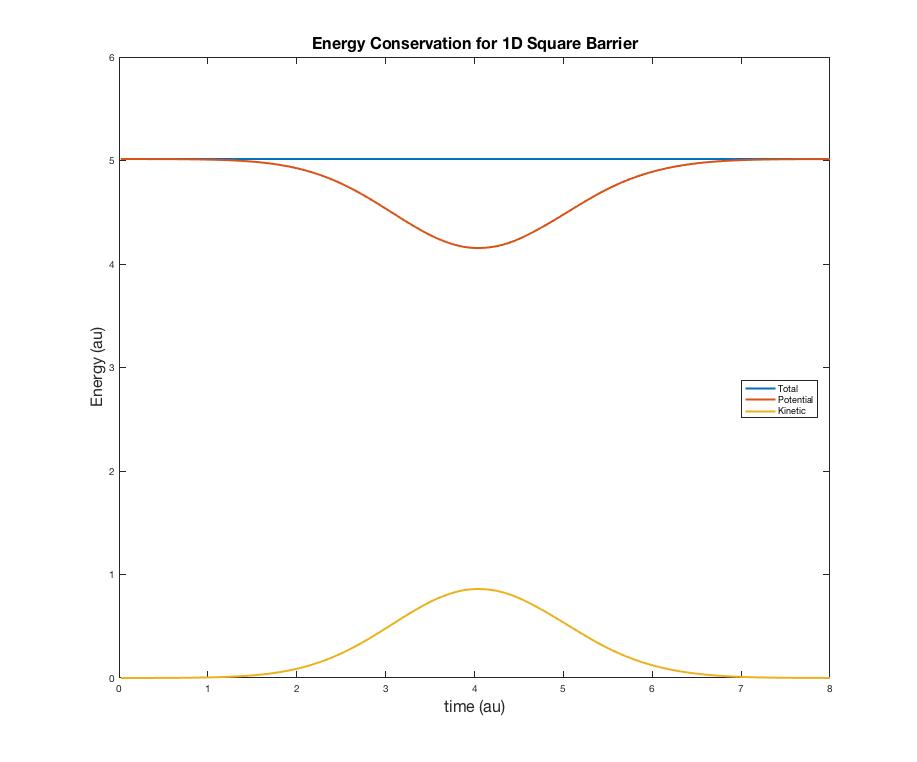
\includegraphics[scale=0.32]{energyPlot.jpg}
\caption{}
\end{figure}

\begin{figure}[!htbp]
\centering
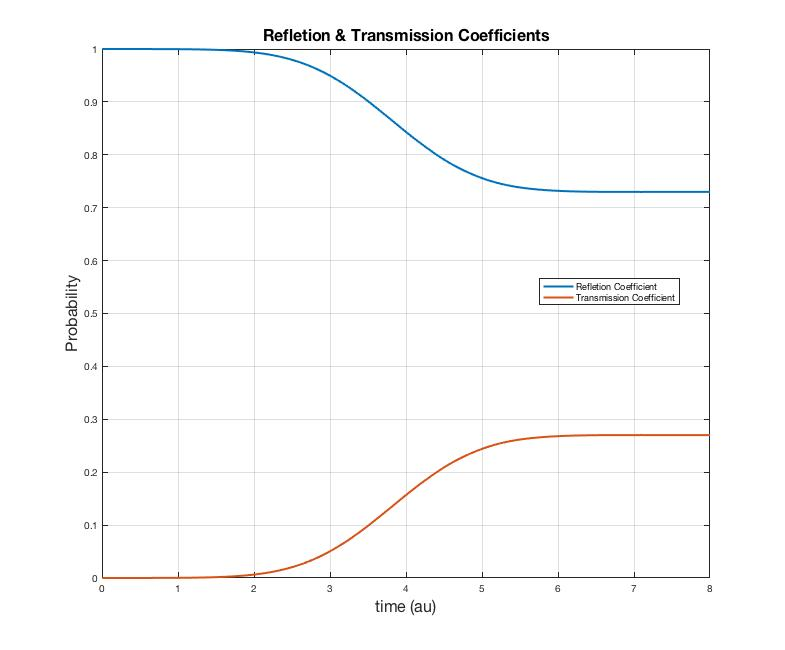
\includegraphics[scale=0.37]{coeffPlot.jpg}
\caption{}
\end{figure}

The reflection and transmission coefficients were plotted as shown in figure 2.

\pagebreak
The source code is as shown below.
\lstinputlisting[language=C, frame=single]{qd1Spectral.c}


\end{document}